\documentclass[12pt,a4paper]{article}

\usepackage[T1]{fontenc}
\usepackage{amsmath, amssymb, amsfonts}
\usepackage[magyar]{babel}
\usepackage[utf8]{inputenc}
\usepackage{graphicx}
\usepackage{graphics}
\usepackage{mathtools}
\usepackage{epsfig}
\usepackage{epstopdf}
\usepackage{cite}
\usepackage{caption}
\usepackage{hyperref}
\usepackage[bottom=4cm]{geometry}
%\geometry{a4paper, portrait, margin=1in}

\title{\huge{Alkalmazott Fizikai Módszerek Laboratórium}\\ \vspace{20pt}
\textbf{Egykristály röntgen diffrakció}}

\author{\Large{\textsc{Csörnyei Géza}} \vspace{10pt}\\
	\textrm{Eötvös Loránd Tudományegyetem}\\
	\textrm{Fizikus MSc I}
	}
\date{}
%\lhead{}
\begin{document}
\addtolength{\voffset}{-1.0cm}
\addtolength{\textheight}{1.0cm}
\begin{titlepage}
\maketitle

\begin{figure}[!htb]
\centering

\includegraphics[scale=0.6]{eltecimer.jpg}
\end{figure}

\hfil \Large{'E' mérőcsoport}\hfil  \\
\vspace*{2pt}
\hfil \Large{\emph{Mérés dátuma:} 2019.10.04.}\hfil \\
\vspace*{2pt}
\hfil \hspace*{45pt} \Large{\emph{Mérés vezetője:} Kovács Zsolt}\hfil
\thispagestyle{empty}
\end{titlepage}

\section{Mérés célja}
\hspace*{10pt} Mérésünk célja különböző egykristály szerkezetek orientációjának meghatározása volt Laue-módszer segítségével. A mérésünk során egy szilícium, egy sókristály, valamint egy alumínium mintával dolgoztunk.

\section{Rövid elméleti összefoglaló}
\hspace*{10pt} Egykristály szerkezetek orientációjának meghatározására kifejlesztett legegyszerűbb és legáltalánosabb módszer a Laue-módszer. A módszer lényege, hogy a minták egy keskeny, folytonos spektrumú röntgensugárzással világítjuk meg, majd a keletkező diffrakciós csúcsokat egy imaging plate segítségével detektáljuk. A detektáló felület helyzetétől függően beszélhetünk első, illetve hátsó reflexiós geometriáról. Mérésünk során az imaging plate a minta és a röntgenforrás között helyezkedett el, vagyis hátsó reflexiós geometriát alkalmaztunk. A folytonos spektrum előnye, hogy ekkor minden nem túl kicsi rácsperiódussal rendelkező síksereg talál magának olyan hullámhosszú összetevőt, mellyel teljesül a Bragg-feltétel:
\begin{equation}
2d_{hkl}\sin\Theta_{hkl}=\lambda,
\end{equation}
ahol $hkl$ a Miller indexek, $d_{hkl}$ az ezekhez tartozó rácssíktávolság, $\Theta_{hkl}$ a Bragg-szög, $\lambda$ pedig a röntgensugár hullámhossza. A diffrakciót szenvedett, reflektált nyalábok irányából meghatározható a reflektáló síksereg normálisának iránya is, ezt írja le a Laue-feltétel, mely a Bragg-törvénnyel ekvivalens:
\begin{equation}
\mathbf{k}-\mathbf{k_0}=\mathbf{g},
\end{equation}
ahol $\mathbf{g}$ a diffrakciós vektor, $\mathbf{k}$ és $\mathbf{k_0}$ a primer és szórt nyalábok hullámszámvektorai. Ez alapján a különböző diffrakciós foltok helyzeteiből meghatározható a hozzájuk tartozó síkok normálisai által bezárt szögek, amelyekből a kristályrendszerhez és a szimmetriákhoz tartozó lehetséges szögértékekkel kiszámítható a minta orientációja.

\section{Mérés menete}
\hspace*{10pt} A mérések során hátsó reflexiós geometriával dolgoztunk és egy keskeny, folytonos spektrumú röntgennyalábot használtunk a minta megvilágítására. A mintát egy goniométerre helyeztük, melynek imaging plate-től vett távolsága és orientációja is változtatható volt. A minta távolságát a mérések során ~40 mm-re állítottuk. A röntgensugárzást 40 kV gyorsítófeszültséggel és 30 mA árammal hoztuk létre egy kobalt röntgencső segítségével. Az egyes minták esetében fél órás expozíciós időt alkalmaztunk. A mérések után a imaging plate-ket kiolvastuk, majd a kapott ábrákat egy külön erre a célra írt programmal, az Orient Expressel dolgoztuk fel. Az egyes ábrákon a diffrakciós pontok jobb láthatósága érdekében küszöbérték transzformációkat hajtottam végre GIMP program segítségével.\\
\hspace*{10pt} Az Orient Express programon belül először kalibráltuk az ábrát az imaging plate tartó árnyékának segítségével (melynek valós hossza 93.81 mm volt; ennek segítségével meghatároztuk a programban a pixelenkénti fizikai hosszt), majd megadtuk az elrendezés paramétereit, majd a vizsgált minta paramétereit. Ezek után a programon belül kiválasztottunk az ábrán néhány kicsi Miller indexekkel rendelkező diffrakciós foltot, amely alapján számítani tudtuk az orientációt. A program több lehetséges orientációt is felajánlott, ezek közül a diffrakciós pontok egyezése alapján választottuk ki a legjobbat.\\
\hspace*{10pt} Az orientáció meghatározása után a programmal kiszámítottuk a minta sztereografikus vetületét a mérési elrendezéshez tartozó orientációban, majd az ábrát a megfelelő szögek megadásával elforgattuk, így megkaptuk az általunk választott irányhoz tartozó elforgatási szögeket.

\section{Kiértékelés}
\subsection{\emph{Si} lapka}
\hspace*{10pt} Méréseinket először a \emph{Si} lapka diffrakciós képének felvételével kezdtük. A mérés beállítása a fentebb felsoroltaknak feleltek meg, az expozíciós idő 30 perc volt. A imaging plate kiolvasását követően kapott ábra a \ref{si:unproc}. ábrán látható.\\
\begin{figure}[!h]
\centering
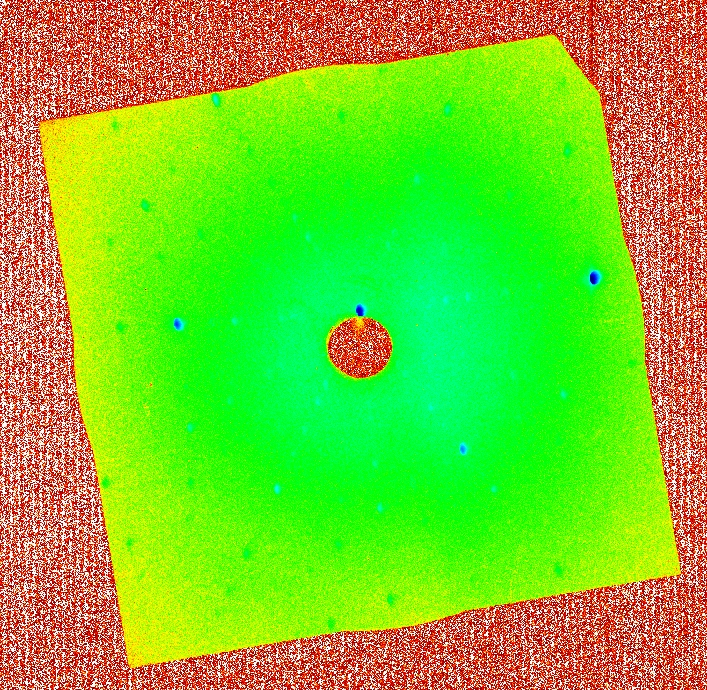
\includegraphics[scale=0.4]{Si}
\caption{A \emph{Si} lapka imaging plate kiolvasása}
\label{si:unproc}
\end{figure}
\newpage
A jobb láthatóság érdekében a kapott képet \texttt{GIMP 2} programban előkészítettem a kiértékeléshez, mely előkészítés során kiemeltem azt a színkomponenst, amelyben a diffrakciós foltok a legjobban látszódtak, majd különböző küszöbérték, görbézési, valamint geometriai változtatásokat (forgatás, tükrözés) alkalmaztam, ezzel kapva a \ref{fig:siproc}. ábrán látható képet.\\
\begin{figure}[!h]
\centering
\includegraphics[scale=1.8]{Si_proc}
\caption{A \emph{Si} lapka diffrakciós képének javított változata. Az egyes indexek az orientáció meghatározásához használt pontokat jelölik}
\label{fig:siproc}
\end{figure}
\newline
A kapott képet betöltöttem az \emph{OrientExpress} programba, majd beimportáltam a \emph{Si} egykristály szerkezetére vonatkozó adatokat, megadtam az imaging plate távolságát, valamint kalibráltam a képen látható, pixelben mért távolságokat az imaging plate szélességének valóságos hosszával, mely 93.81 mm volt. Ezen értékek megadása után kijelöltem az indexeléshez használni kívánt pontokat (\ref{fig:siproc}. ábra), majd a program megadta a lehetséges indexeléseket. A legmegfelelőbbnek választott indexelés, valamint az egyes pontok koordinátái (a kép középpontjától mért távolságok) láthatók a \ref{tab:si}. táblázatban.\\
\begin{table}[!h]
\begin{center}
\begin{tabular}{|c|c|c|c|}
\hline
Index & X [cm] & Y [cm] & \emph{hkl} \\
\hline
1 & 0.63 & 0.14 & ${\overline{1}\overline{1}\overline{1}}$\\
\hline
2 & 0.89 & -3.00 & ${\overline{2}\overline{1}\overline{1}}$\\
\hline
3 & -2.00 & 1.46 & ${\overline{1}\overline{1}\overline{2}}$\\
\hline
4 & -2.17 & -1.78 & ${\overline{3}\overline{1}\overline{3}}$\\
\hline
\end{tabular}
\caption{A \emph{Si} lapka indexeléséhez használt pontok koordinátái}
\label{tab:si}
\end{center}
\end{table}
\newline
A kapott indexelés esetére végrehajtottam a sztereografikus projekció lépést az \emph{OrientExpress} segítségével, melyből a \ref{si:stereo}. ábrát kaptam. A képen a középpont a nyaláb irányának felel meg.\\
\begin{figure}[!h]
\centering
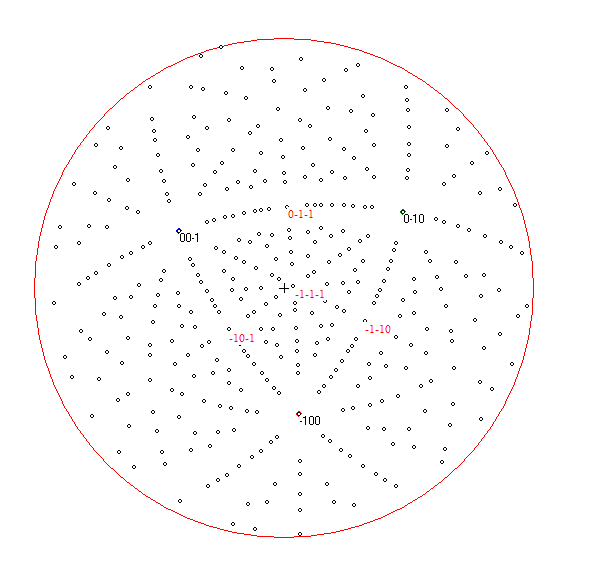
\includegraphics[scale=1.8]{SI_sztereo_nonorient}
\caption{A $Si$ lapka diffrakciós képének sztereografikus projekciója}
\label{si:stereo}
\end{figure}
\newline
A minta orientációjának meghatározásának meghatározásához be kellett forgatnunk ezt a projekciót egy tetszőleges irányba, mely irányt én ${\overline{1}\overline{1}\overline{1}}$-nek választottam. A már orientált sztereografikus projekció a \ref{fig:si_orient}. ábrán látható.\\
\begin{figure}[!h]
\centering
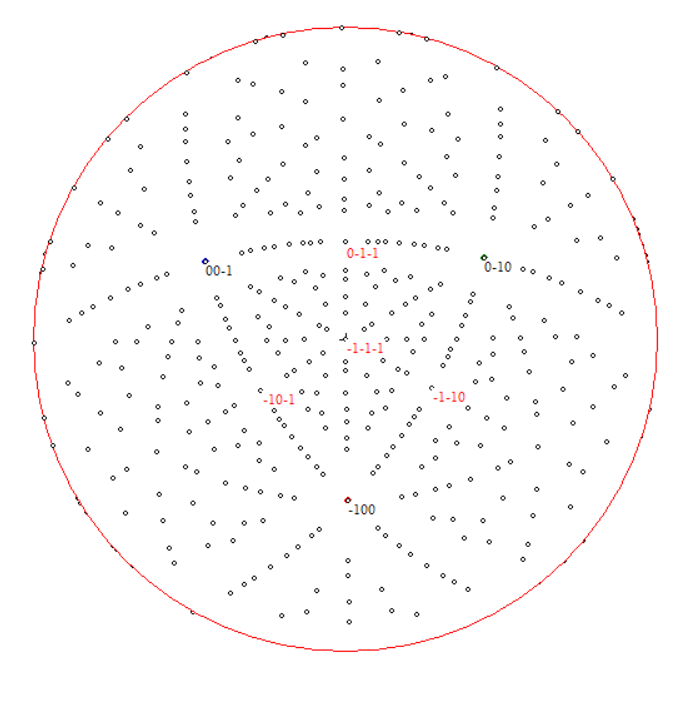
\includegraphics[scale=1.6]{SI_sztereo_oriented}
\caption{A \emph{Si} lapka sztereografikus projekciójának orientált (beforgatott) változata}
\label{fig:si_orient}
\end{figure}
\newline
Az egyes forgatási szögek (a programbeli tengelyek körül, a nekik megfelelő jelöléssel):\\
\begin{itemize}
\item{X=3.0$^{\circ}$}
\item{Y=1.5$^{\circ}$}
\item{Z=-5.0$^{\circ}$}
\end{itemize}

Mivel a mintát lapjával párhuzamosan rögzítettük a mintatartóra és ilyen kicsi szögekkel kellett csak elforgatnunk a projekciót, hogy beálljuk egy kristálytani irányba, ezért kijelenthető, hogy a minta jó közelítéssel egyik kristálysíkja mentén lett elvágva.

\subsection{\emph{NaCl} kristály}
\hspace*{10pt} A kiértékelés lépései és a mérési elrendezés az előzővel azonos volt. A minta diffrakciós felvétele:\\
\begin{figure}[!h]
\centering
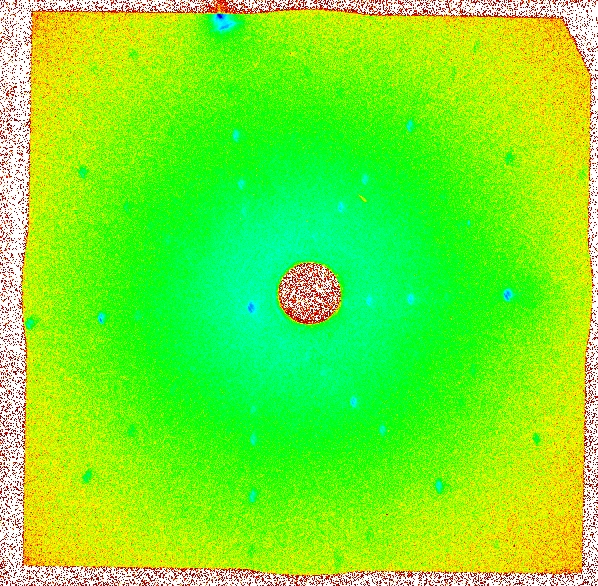
\includegraphics[scale=0.4]{NaCl}
\caption{A \emph{NaCl} minta imaging plate kiolvasása}
\label{nacl:unproc}
\end{figure}
\newline
A kapott képet hasonlóan előkészítettem (\ref{fig:nacl_proc}. ábra), majd elvégeztem a programmal az indexelés lépést (\ref{tab:nacl}. táblázat). \\

\begin{figure}[!h]
\centering
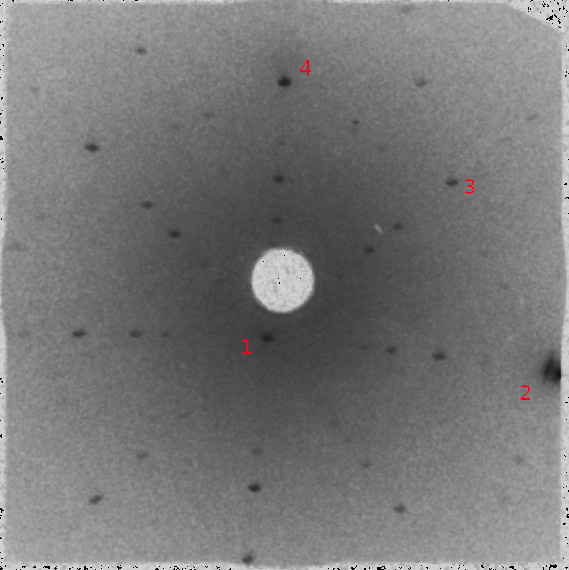
\includegraphics[scale=1.8]{nacl_proc}
\caption{A \emph{NaCl} minta diffrakciós képének javított változata. Az egyes indexek az orientáció meghatározásához használt pontokat jelölik}
\label{fig:nacl_proc}
\end{figure}

\begin{table}[!h]
\begin{center}
\begin{tabular}{|c|c|c|c|}
\hline
Index & X [cm] & Y [cm] & \emph{hkl} \\
\hline
1 & -0.21 & -0.97 & ${\overline{1}00}$\\
\hline
2 & 4.65 & -1.50 & ${\overline{2}\overline{1}0}$\\
\hline
3 & 2.97 & 1.69 & ${\overline{3}\overline{1}\overline{1}}$\\
\hline
4 & 0.05 & 3.40 & ${\overline{2}0\overline{1}}$\\
\hline
\end{tabular}
\caption{A \emph{NaCl} minta indexeléséhez használt pontok koordinátái}
\label{tab:nacl}
\end{center}
\end{table}
\newpage
A minta orientációjának meghatározásához itt is elvégeztem a sztereografikus projekciót a korábbihoz hasonló módon. Az eredmény a \ref{fig:nacl_sztereo}. ábrán látható.\\

\begin{figure}[!h]
\centering
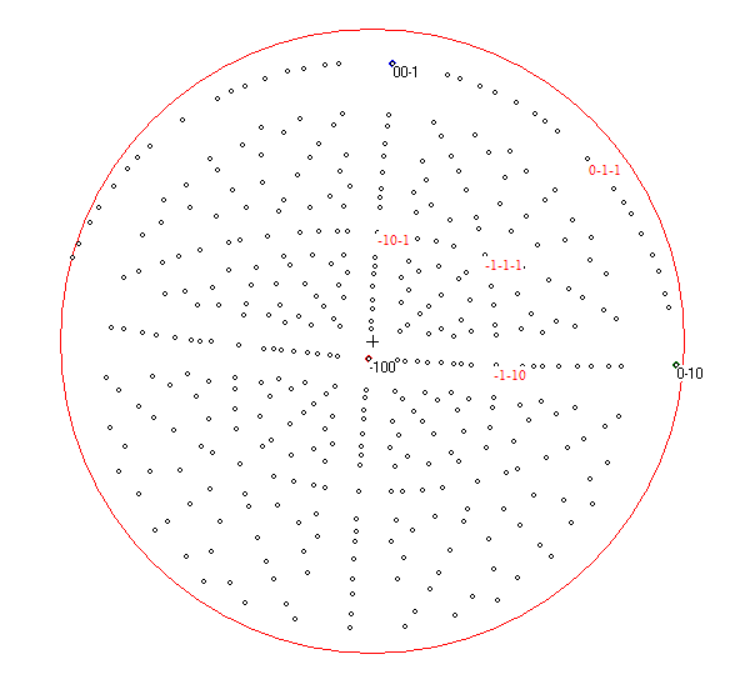
\includegraphics[scale=1.4]{nacl_sztereo}
\caption{A $NaCl$ kristály diffrakciós képének sztereografikus projekciója}
\label{fig:nacl_sztereo}
\end{figure}

A korábbihoz hasonlóan ezen a képen is elvégeztem az orientálás lépést, azaz beforgattam a rendszert a 
${\overline{1}\overline{1}\overline{1}}$ irányba (\ref{fig:nacl_oriented}. ábra).\\

\begin{figure}[!h]
\centering
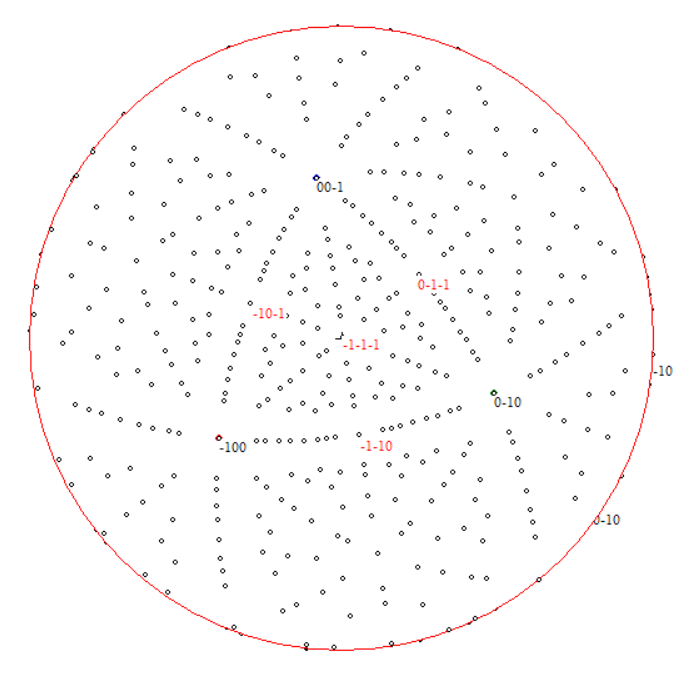
\includegraphics[scale=1.4]{nacl_orient}
\caption{A \emph{NaCl} minta sztereografikus projekciójának orientált (beforgatott) változata}
\label{fig:nacl_oriented}
\end{figure}

A beforgatáshoz szükséges szögek a korábbi jelöléseknek megfelelően:
\begin{itemize}
\item{X=13.0$^{\circ}$}
\item{Y=25.0$^{\circ}$}
\item{Z=43.0$^{\circ}$}
\end{itemize}

\subsection{\emph{Al} minta}
\hspace*{10pt} A mérés során az alumínium mintát vizsgáltuk meg utoljára. A beállítások a korábbiaknak megfelelőek voltak, az expozíciós idő itt is 30 perc volt. Az imaging plate kiolvasása után kapott diffrakciós kép a \ref{fig:al}. ábrán látható.\\
\newpage
\begin{figure}
\centering
\includegraphics[scale=0.4]{al}
\caption{Az alumínium minta diffrakciós képe}
\label{fig:al}
\end{figure}

A fenti ábrán végrehajtottam ugyanazon transzformációkat mint korábban, az eredmény az indexeléssel a \ref{fig:al_proc}. ábrán látható. Az egyes indexelt pontok koordinátái a \ref{tab:al}. táblázatban találhatók.
\begin{figure}[!h]
\centering
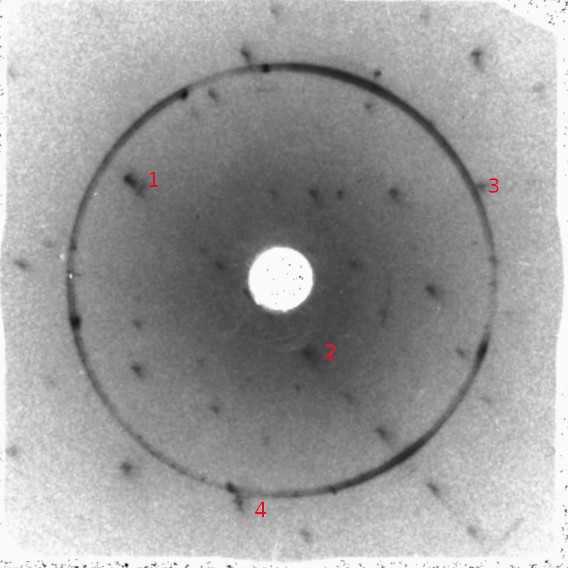
\includegraphics[scale=1.8]{al_proc}
\caption{A \emph{Al} minta diffrakciós képének javított változata. Az egyes indexek az orientáció meghatározásához használt pontokat jelölik}
\label{al:proc}
\end{figure}
\newpage
\begin{table}[!h]
\begin{center}
\begin{tabular}{|c|c|c|c|}
\hline
Index & X [cm] & Y [cm] & \emph{hkl} \\
\hline
1 & -2.56 & 1.77 & ${\overline{3}12}$\\
\hline
2 & 3.49 & 1.62 & ${\overline{1}21}$\\
\hline
3 & 0.58 & -1.25 & ${011}$\\
\hline
4 & -0.64 & -3.83 & ${\overline{1}10}$\\
\hline
\end{tabular}
\caption{Az \emph{Al} minta indexeléséhez használt pontok koordinátái}
\label{tab:al}
\end{center}
\end{table}
A kapott sztereografikus projekció a \ref{al_sztereo}. ábrán látható.\\

\begin{figure}[!h]
\centering
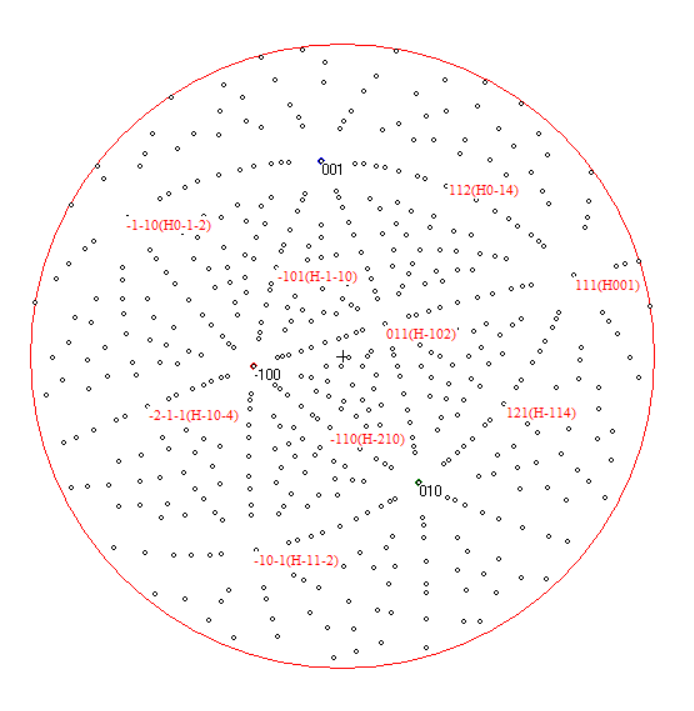
\includegraphics[scale=1.4]{al_sztereo}
\caption{Az $Al$ minta diffrakciós képének sztereografikus projekciója}
\label{fig:al_sztereo}
\end{figure}
\newpage
A korábbiakhoz hasonlóan itt is elvégeztem a minta orientálását, ennek megfelelően az orientált sztereografikus projekció:\\
\begin{figure}[!h]
\centering
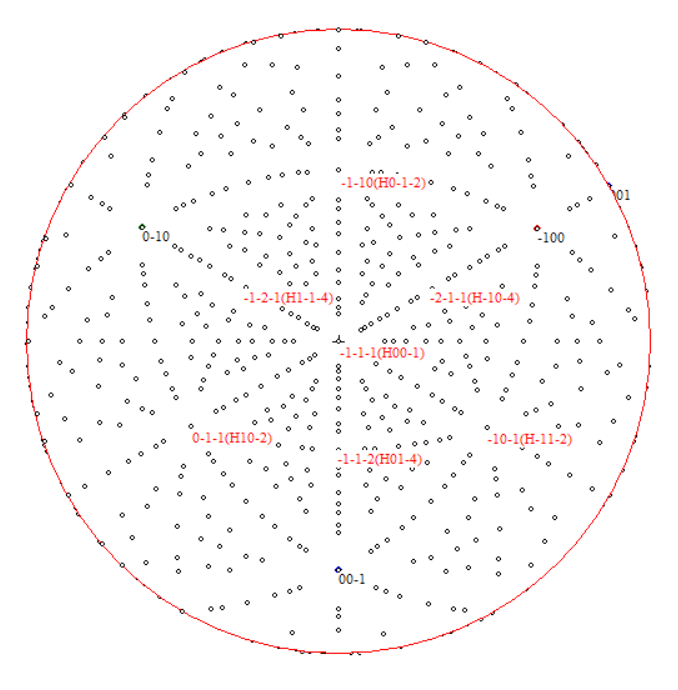
\includegraphics[scale=1.4]{al_orient}
\caption{Az \emph{Al} minta sztereografikus projekciójának orientált (beforgatott) változata}
\label{fig:al_oriented}
\end{figure}
\
A beforgatáshoz szükséges szögek a korábbi jelöléseknek megfelelően:
\begin{itemize}
\item{X=25.0$^{\circ}$}
\item{Y=-22.0$^{\circ}$}
\item{Z=-105.0$^{\circ}$}
\end{itemize}

\section{Diszkusszió}
\hspace*{10pt} Mérésünk során megismerkedtünk a Laue-módszerrel, valamint az ahhoz használatos eszközökkel, valamint sikeresen meghatároztuk három különböző minta orientációját.
\end{document}